% 2005_jiangsu_q19_fig1: two unit circles O1=(-2,0), O2=(2,0); representative P=(1,2.828427) on locus; M/N computed tangent points.
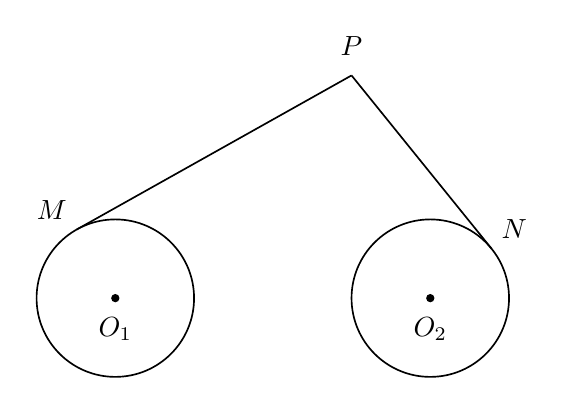
\begin{tikzpicture}[x=1cm,y=1cm,line width=.6pt,font=\normalsize]
\coordinate (O1) at (-2,0);
\coordinate (O2) at (2,0);
\coordinate (P) at (1,2.828427);
\coordinate (M) at (-2.489042,0.872260);
\coordinate (N) at (2.777778,0.628539);
\draw (O1) circle[radius=1cm];
\draw (O2) circle[radius=1cm];
\draw (P)--(M);
\draw (P)--(N);
\fill (O1) circle (1.5pt);
\fill (O2) circle (1.5pt);
\node[below] at (-2,-0.12) {$O_{1}$};
\node[below] at (2,-0.12) {$O_{2}$};
\node[above] at (1,2.95) {$P$};
\node[above left] at (-2.489042,0.872260) {$M$};
\node[above right] at (2.777778,0.628539) {$N$};
\end{tikzpicture}
